\documentclass[aspectratio=169]{beamer}
\usepackage{will_handley_beamer}
\usepackage{title_page}
\newcommand{\av}[2][]{\left\langle #2\right\rangle_{#1}}
\newcommand{\student}[3]{
    \tikz[overlay,remember picture]{
        \node[anchor=north east] (A) at ($(current page.north east)+(0,0)$) {\includegraphics[width=0.09\textheight]{figures/students/#1}};
        \node[anchor=north east] (B) at (A.north west) {#2};
        \node[anchor=north east] (B) at (B.south east) {\tiny #3};
    }
    \vspace{-0.1\textheight}
}

% Commands
% --------
% - \arxiv{arxiv number}
% - \cols{width}{lh column}{rh column}
% -  \begin{fig(left|right)}[fractional width (e.g 0.6) ]{name of image}
%        content of other column
%    \end{fig(left|right)}

% Talk details
% ------------
\title{REACH: Nested sampling tools}
%\subtitle{<+subtitle+>}
\date{26\textsuperscript{th} September 2023}

\begin{document}

\begin{frame}
    \titlepage
\end{frame}

\begin{frame}
    \frametitle{What do we use nested sampling for?}
        Given a (scalar) function $f$ with a vector of parameters $x$, nested sampling can be used for:
    \vspace{-10pt}
    \begin{columns}[t]
        \column{0.3\textwidth}
        \begin{block}{Optimisation}
            \[x_\text{max} = \max_x{f(x)}\]
            \hfill \emph{Experimental design}
        \end{block}
        \column{0.3\textwidth}
        \begin{block}{Exploration}
            \vspace{-10pt}
            \[\text{draw/sample}\quad x\sim f\]
            \hfill \emph{Parameter estimation}
        \end{block}
        \column{0.3\textwidth}
        \begin{block}{Integration}
            \[\int f(x) dV \]
            \hfill \emph{Model comparison}
        \end{block}
    \end{columns}
    \begin{columns}[t]
        \column{0.33\textwidth}
        \centerline{\includegraphics[width=0.8\textwidth,page=13]{figures/himmelblau}}
        \column{0.33\textwidth}
        \centerline{\includegraphics[width=0.8\textwidth,page=15]{figures/himmelblau}}
        \column{0.33\textwidth}
        \centerline{\includegraphics[width=0.8\textwidth,page=14]{figures/himmelblau}}
    \end{columns}
\end{frame}

\begin{frame}
    \frametitle{The nested sampling meta-algorithm: live points}
    \begin{columns}
        \column{0.5\textwidth}
        \begin{itemize}
            \item Start with $n$ random samples over the space.
            \item Delete outermost sample, and replace with a new random one at higher integrand value.
            \item The ``live points'' steadily contract around the peak(s) of the function.
            \item We can use this evolution to estimate volume \emph{probabilistically}.
            \item At each iteration, the contours contract by $\sim\frac{1}{n}\only<9->{\pm \frac{1}{n}}$ of their volume.
            \item This is an exponential contraction, so
                \[  \int f(x) dV \approx \sum_i f(x_i) \Delta V_i, \quad V_i = V_0 e^{-\only<9->{(}i\only<9->{\pm\sqrt{i})}/n} \]
%            \item Nested sampling: completely different way to scan.
%            \item Ensemble sampling compresses entire space$\to$peak(s).
%            \item Sequentially update a set $S$ of $n$ samples:
%                \begin{itemize}
%                    \item[$S_0$:]  Generate $n$ samples uniformly over the space (from a measure $\pi$). 
%
%                    \item[$S_{i+1}$:] Delete the lowest likelihood sample in $S_{i}$, and replace it with a new uniform sample with higher likelihood.
%                \end{itemize}
%            \item Requires one to be able to sample uniformly within a region, subject to a {\em hard constraint}:
%                \[\{\theta\sim \pi : \mathcal{L}(\theta)>\mathcal{L}_*. \}\]
%            \item This procedure optimises (multimodally), and can calculate the \C[3]{evidence}/integral of function \& \C[0]{posterior}/sample weights.
        \end{itemize}
        \column{0.5\textwidth}
        \includegraphics<1|handout:0>[width=\textwidth,page=1]{figures/himmelblau}%
        \includegraphics<2|handout:0>[width=\textwidth,page=2]{figures/himmelblau}%
        \includegraphics<3|handout:0>[width=\textwidth,page=3]{figures/himmelblau}%
        \includegraphics<4|handout:0>[width=\textwidth,page=4]{figures/himmelblau}%
        \includegraphics<5|handout:0>[width=\textwidth,page=5]{figures/himmelblau}%
        \includegraphics<6|handout:0>[width=\textwidth,page=6]{figures/himmelblau}%
        \includegraphics<7|handout:0>[width=\textwidth,page=7]{figures/himmelblau}%
        \includegraphics<8-         >[width=\textwidth,page=8]{figures/himmelblau}%
    \end{columns}
\end{frame}

\begin{frame}
    \frametitle{The nested sampling meta-algorithm: dead points}
    \begin{columns}
        \column{0.5\textwidth}
        \begin{itemize}
            \item At the end, one is left with a set of discarded ``dead'' points.
            \item Can be weighted to form posterior samples, prior samples, or anything in between.
            \item Nested sampling estimates the \textbf{density of states} and calculates partition functions
                \[Z(\beta) = \sum_i f(x_i)^\beta \Delta V_i.\]
            \item The evolving ensemble of live points allows:
                \begin{itemize}
                    \item implementations to self-tune
                    \item exploration of multimodal functions
                    \item global and local optimisation
                \end{itemize}
            %\item Interpreted as a Bayesian algorithm, it
            %    \begin{itemize}
            %        \item Computes the Bayesian evidence (model comparison)
            %        \item Produces (weighted) posterior samples (parameter estimation)
            %    \end{itemize}
        \end{itemize}
        \column{0.5\textwidth}
        \includegraphics[width=\textwidth,page=14]{figures/himmelblau}%
        %\includegraphics<1|handout:0>[width=\textwidth,page=14]{figures/himmelblau}%
        %\includegraphics<2          >[width=\textwidth,page=15]{figures/himmelblau}%
    \end{columns}
\end{frame}

\begin{frame}
    \frametitle{Dead measure}
    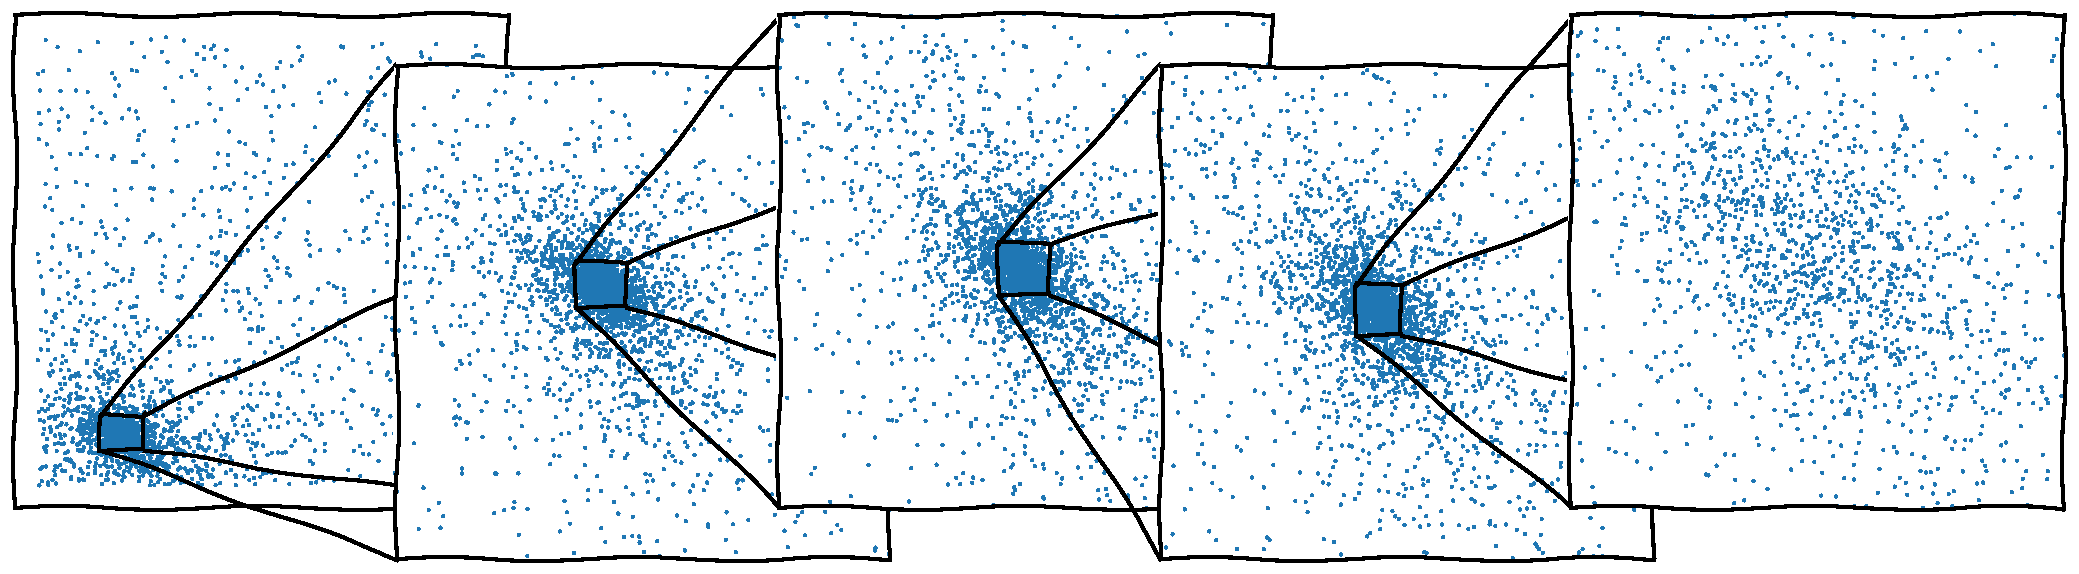
\includegraphics[width=\textwidth]{figures/dead_measure}
    \begin{columns}
        \column{0.69\textwidth}
        \begin{itemize}
            \item Dead points have a unique scale-invariant distribution $\propto\: \tfrac{dV}{V}$.
            \item Uniform over original region, exponentially concentrating on region of interest (until termination volume).
            \item Full coverage of tails enables integration.
            \item Good for training emulators (HERA~\arxiv{2108.07282}).
        \end{itemize}
        \column{0.3\textwidth}
        \begin{block}{Applications}
        \begin{itemize}
            \item training emulators.
            \item gridding simulations
            \item beta flows\ldots
            \item good name for a band
        \end{itemize}
        \end{block}
    \end{columns}
\end{frame}

\begin{frame}
    \frametitle{Applications: The three pillars of Bayesian inference}
    \vspace{-20pt}
    \begin{columns}[t]
        \column{0.33\textwidth}
        \begin{block}{Parameter estimation}
            What do the data tell us about the parameters of a model?

            \textit{e.g. the central frequency $\nu_0$ of Gaussian global signal}
            \[ \hspace{-4pt}\C[0]{P(\theta|D,M)} = \frac{\C[2]{P(D|\theta,M)} \C[1]{P(\theta|M)}}{\C[3]{P(D|M)}} \] 
            \[ \C[0]{\mathcal{P}} = \frac{\C[2]{\mathcal{L}} \times\C[1]{\pi}}{\C[3]{\mathcal{Z}}}\] 
            \[ \C[0]{\text{Posterior}} = \frac{\C[2]{\text{Likelihood}} \times\C[1]{\text{Prior}}}{\C[3]{\text{Evidence}}}\]
        \end{block}
        \column{0.3\textwidth}
        \begin{block}{Model comparison}
            How much does the data support a particular model?

            \textit{e.g. $\Lambda$CDM vs cosmic strings}
            \[ \C[4]{P(M|D)} = \frac{\C[3]{P(D|M)} \C[5]{P(M)}}{\C[7]{P(D)}} \vspace{-7pt}\]
            \[ \frac{\C[3]{\mathcal{Z}_\mathcal{M}} \C[5]{\Pi_\mathcal{M}}}{\C[7]{\sum_m Z_m \Pi_m}} \]
            \[ \C[4]{\text{Posterior}} = \frac{\C[3]{\text{Evidence}} \times\C[5]{\text{Prior}}}{\C[7]{\text{Normalisation}}}\]
        \end{block}
        \column{0.33\textwidth}
        \begin{block}{Tension quantification}
            Do different datasets make consistent predictions from the same model? 
            \textit{e.g. SARAS vs EDGES}
            \[ \mathcal{R} = \frac{\C[3]{\mathcal{Z}}_{AB}}{\C[3]{\mathcal{Z}}_A\C[3]{\mathcal{Z}}_\mathcal{B}}\] 
            \[
                \begin{aligned} \log\mathcal{S} = \av[{\C[0]{\mathcal{P}}_{AB}}]{\C[2]{\log\mathcal{L}}_{AB}}&\\
                    -\av[{\C[0]{\mathcal{P}}_{A}}]{\C[2]{\log\mathcal{L}}_{A}}&\\
                    -\av[{\C[0]{\mathcal{P}}_{B}}]{\C[2]{\log\mathcal{L}}_{B}}&
                \end{aligned}
            \]
        \end{block}
    \end{columns}
    \begin{itemize}
        \item Note, REACH has been a powerful ambassador for ``model'' involving theory, systematics and inference parameters~\arxiv{2204.04491}
    \end{itemize}
\end{frame}


\begin{frame}
    \frametitle{\texttt{anesthetic}: the nested sampling toolkit}
    \begin{itemize}
        \item 
    \end{itemize}<++>

\end{frame}

\begin{frame}
    \frametitle{Likelihood-free inference (aka SBI)}
\student{kilian_scheutwinkel}{Kilian Scheutwinkel}{PhD}

    \vspace{10pt}
    \begin{columns}
        \column{0.5\textwidth}
        \vspace{-10pt}
        \begin{itemize}
            \item How do you do inference if you don't know the likelihood $P(D|\theta)$?
                \begin{itemize}
                    \item e.g.\ if you can simulate a disease outbreak, how can you infer a posterior on $R_0$, or select the most predictive model?
                \end{itemize}
            \item If you can forward simulate/model $\theta\to D$, then you have an implicit likelihood.
            \item LFI aims to (machine-)\emph{learn} the likelihood from forward simulations $\{(\theta,D)\}$.
            \item Nested sampling has much to offer
                \begin{itemize}
                    \item truncation strategies (\texttt{PolySwyft})
                    \item evidence driven compression
                    \item marginalised machine learning
                \end{itemize}
            \item In my view, LFI represents the future of inference -- in twenty years time this will be as well-used as MCMC techniques are today.
        \end{itemize}
        \column{0.5\textwidth}
        \includegraphics[width=\textwidth]{figures/noisy.pdf}
        \includegraphics[width=\textwidth]{figures/three_ways_II.pdf}
    \end{columns}
\end{frame}

% What could we do better in antenna design in future?
% multiobjective optimisation
% evidence networks

\end{document}
